\sigma_.L\section{Auswertung}
\label{sec:Auswertung}


Die Graphen wurden sowohl mit Matplotlib \cite{matplotlib} als auch NumPy \cite{numpy} erstellt. Die
Fehlerrechnung wurde mithilfe von Uncertainties \cite{uncertainties} durchgeführt.

\subsection{Apparatekonstanten}
Für die Messreihen wurde Gerät 2 verwendet.
Die Werte für Induktivität $L$ der Spule, die Kapazität $C$ und den verwendeten Widerstand $R_.1$ befinden sich in Tabelle \ref{tab:tab1}

\begin{table}
	\centering
	\caption{Apparatekonstanten}
\label{tab:tab1}
	\sisetup{table-format=1.2}
	\begin{tabular}{S[table-format=1.2]S[table-format=1.3]S[table-format=2.1]}
		\toprule
		{$L/ 10^3 \si{\hertz}$} & {$C/10^9\si{\farad}$} & {$R/\si{hertz}$} \\
		\midrule
		${10,11\pm 0,03}$ & ${2,098\pm 0,006}$ & ${48,1\pm 0,1}$ \\
		\bottomrule
	\end{tabular}
\end{table}
\subsection{Abklingzeit und effektiver Dämpfungswiderstand}
In Tabelle \ref{tab:tab2} sind die Messwerte des in Abbildung \ref{fig:abb1} sichtbaren Graphen zu sehen.\newline
Als Generatorspannung wurde eine Rechteckspannung von $U_.G=20V$ verwendet.
\begin{table}
	\centering
	\caption{Apparatekonstanten}
\label{tab:tab2}
	\sisetup{table-format=1.2}
	\begin{tabular}{S[table-format=3.0]S[table-format=2.1]}
		\toprule
		{$t/10^6\si{\second}$} & {$U_.C/\si{\volt}$} \\
		\midrule
		0 & 19.4 \\
		30 & 16.0 \\
		60 & 13.4 \\
		90 & 11.2 \\
		120 & 9.6 \\
		150 & 8.0 \\
		180 & 7.0 \\
		210 & 5.8 \\
		240 & 4.8 \\
		270 & 4.0 \\
		300 & 3.6 \\
		330 & 3.0 \\
		360 & 2.6 \\
		390 & 2.2 \\

		\bottomrule
	\end{tabular}
\end{table}
\begin{figure}
\centering
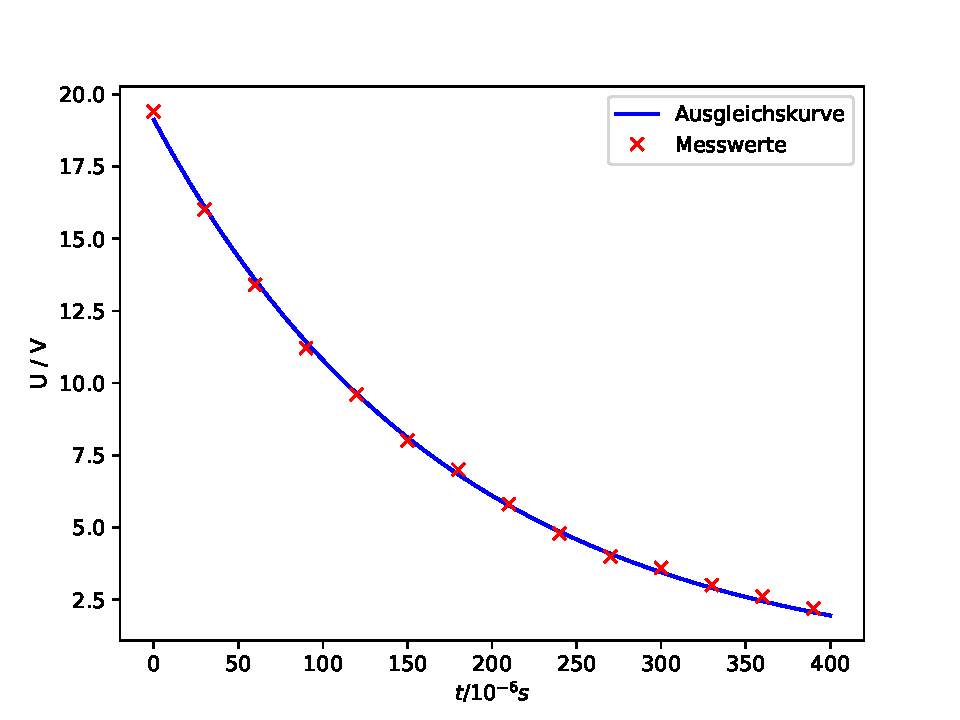
\includegraphics[scale=0.6]{content/images/a.pdf}
\caption{Messdaten eines Abklingvorgangs eines RLC-Schwingkreises}
\label{fig:abb1}
\end{figure}
\newpage
\noindent Die Regression $U(t)=A_.0e^{-2\pi\mu t}$ liefert:
\begin{align}
A_.0 &= \SI{19,11(12)}{\volt} \\
\mu &= \SI{909(9)}{\hertz}
\end{align}
Nach Gleichung \eqref{eq:gamma} und \eqref{eq:tau} ergibt sich mit $\gamma=2\pi\mu$:
\begin{align}
R_.{eff}&=\SI{115(1)}{\ohm} \\
\tau &=\SI{175(1)e-6}{\second}
\end{align}
Der Fehler von $R_.{eff}$ errechnet sich dabei aus der Gaußschen Fehlerfortpflanzung
\[
\sigma_.R=\sqrt{(4\pi L\sigma_.{\mu})^2 +(4\pi\mu\siga_.L)^2),
\]
wobei $\sigma_.L$ aus Tabelle \ref{tab:tab1} abzulesen und $\sigma_.{\mu}$ durch die Regression bestimmt wurde.
Analog dazu errechnet sich der Fehler der Abklingzeit $\tau$ zu
\[
\sigma_.{\tau}=\frac{\sigma_.{\mu}}{2\pi\mu^2}
\]
Der berechnete effektive Widerstand $R_.{eff}$ weicht von dem geschalteten Widerstand $R_.1$ um $\Delta R=140\%$ ab.
\subsection{Aperiodischer Grenzfall}
Der Widerstand für den die Schwingung in den aperiodischen Grenzfall übergeht wurde zu
\[
R_.{ap,exp}=\SI{3,5e3}{\ohm}\text{.}
\]
Der aus Gleichung \eqref{eq:} berechnete Wert beträgt
\[
R_.{ap,theo}=\SI{4,390(9)e3}{\ohm},
\]
wobei sich der Fehler aus
\[
\sigma_.{R}=\sqrt(\sigma_.L^2/(CL)+(L\sigma_.C)^2/(C^3L))
\]
berechnet.\newline
Die Abweichung beträgt somit
\[
\Delta R_.[ap}=25,4\%
\]
\subsection{Frequenzabhängigkeit der Kondensatorspannung}
\subsubsection{Frequenzabhängigkeit der Amplitude}
\subsubsection{Frequenzabhängigkeit der Phase}